\subsubsection{补集}

在研究集合与集合之间的关系时,在某些情况下,这些集合都是某一个给定的集合的子集,这个给定的集合可以看作一个\textbf{全集},用符号 $I$ 表示。也就是说,全集含有我们所要研究的各个集合的全部元素。

例如,在研究数集时,常常把实数集 $R$ 作为全集;在研究图形的集合时,常常把所有的空间图形组成的集合作为全集。

已知全集 $I$,集合$A \subseteq I$,由 $I$ 中所有不属于 $A$ 的元素组成的集合,叫做集合 $A$ 在集合 $I$ 中的\textbf{补集},记作 $\bar{A}$(可读作“A补”),即

$$\buji{A} = \{ x \mid x \in I \text{,且} x \notin A \} \text{。}$$


\begin{wrapfigure}{R}{5cm}
    \centering
    \begin{tikzpicture}
        \draw[pattern=lines] (0, 0) rectangle (5,4);
        \begin{scope}
           \draw[fill=white] (3,2) circle (1.2) node{$A$};
        \end{scope}
        \node at (1,2) [fill=white] {$\buji{A}$};
        \node at (0.6,3.5) [fill=white] {$I$};
    \end{tikzpicture}
    \caption{}\label{fig:1-4}
\end{wrapfigure}

图\ref{fig:1-4}中的长方形内表示全集 $I$,圆内表示集合 $A$,阴影部分表示集合 $A$ 在集合 $I$中的补集 $\buji{A}$。

由补集定义容易知道,对于任何集合 $A$,有
$$ A \cup \buji{A} = I, \quad A \cap \buji{A} = \kongji, \quad \buji{\buji{A}} = A \text{,}$$
其中,$\buji{\buji{A}}$ 表示 $\buji{A}$ 在 $I$ 中的补集。

例如,如果 $I = \{1,2,3,4,5,6\}$,$A=\{1,3,5\}$,那么
$$\buji{A} = \{2,4,6\} \text{。}$$

容易看出
\begin{gather*}
    \{1,3,5\} \cup \{2,4,6\} = \{1,2,3,4,5,6\} = I, \\
    \{1,3,5\} \cap \{2,4,6\} = \kongji, \\
    \buji{\buji{A}} = \{1,3,5\} = A \text{。}
\end{gather*}

\liti 已知 $I = R = \{\text{实数}\}$,$Q = \{\text{有理数}\}$,求$\buji{Q}$。

\jie 有理数集在实数集中的补集是全体无理数的集合,所以
$$\buji{Q} = \{\text{无理数}\} \text{。}$$

以后我们就把全体无理数的集合简称为\textbf{无理数集},记作$\buji{Q}$。

\liti 设 $I = \{\text{梯形}\}$,$A = \{\text{等腰梯形}\}$,求$\buji{A}$。

\jie $\buji{A} = \{\text{不等腰梯形}\}$。

\liti 已知 $I = R = \{\text{实数}\}$,$A = \{x \mid x^2+3x+2<0\}$,求$\buji{A}$。

\jie $\because A = \{x \mid x^2+3x+2<0\} = \{x \mid -2<x<-1\}$,

\begin{minipage}{7cm}
    \begin{align*}
        \therefore \buji{A} &= \{x \mid x \leqslant -2\} \cup \{x \mid x \geqslant -1\} \\
                                &= \{x \mid x \leqslant -2 \text{,或} x \geqslant -1\} \text{。}
    \end{align*}
\end{minipage}

\liti 设 $I = \{1,2,3,4,5,6,7,8\}$,$A=\{1,3,5\}$,$B=\{4,7,8\}$,求 $\buji{A}$,$\buji{B}$,$\buji{A} \cap \buji{B}$,$\buji{A} \cup \buji{B}$。

\jie
\begin{minipage}[t]{6cm}
    \gongshishangyi
    \begin{align*}
        &\buji{A} = \{1,2,6,7,8\}, \buji{B} = \{1,2,3,5,6\}, \\
        &\buji{A} \cap \buji{B} = \{1,2,6\}, \\
        &\buji{A} \cup \buji{B} = \{1,2,3,5,6,7,8\} \text{。}
    \end{align*}
\end{minipage}

\lianxi

\begin{xiaotis}

\xiaoti{设 $A=\{1,2,3,4,5\}$,$B=\{4,5,6,7,8,9\}$。}

\begin{xiaoxiaotis}
    
    \xiaoxiaoti{求 $A \cap B$,$A \cup B$。}

    \xiaoxiaoti{用适当的符号($\supset$,$\subset$)填空:\\
        $A \cup B \xhx A, \quad A \cup B \xhx B, \quad A \cap B \xhx A \cup B$。
    }

\end{xiaoxiaotis}

\xiaoti{设 $A = \{x \mid -2<x<1\}$,$B = \{x \mid 0 \leqslant x \leqslant 2\}$,求 $A \cup B$。}

\xiaoti{设 $A = \{x \mid x>-2\}$,$B = \{x \mid x \geqslant 3\}$,求 $A \cup B$。}

\xiaoti{写出不等式 $|a+3|>1$ 的解集并进行化简(提示: $|a+3|>1 \Longleftrightarrow a+3>1 \text{,或} a+3<-1$)。}

\xiaoti{写出不等式 $x^2-x-2<0$ 的解集并进行化简。}

\xiaoti{设 $A=\{\text{直角三角形}\}$,$B=\{\text{斜三角形}\}$},求$A \cup B$。

\xiaoti{已知 $N$ 为自然数集。}
\begin{xiaoxiaotis}
    
    \xiaoxiaoti{如果 $I$ 为整数集 $Z$,求 $\buji{N}$;}

    \xiaoxiaoti{如果 $I$ 为非负整数集,求 $\buji{N}$。}

\end{xiaoxiaotis}

\xiaoti{已知 $I = R = \{\text{实数}\}$,$\buji{Q} = \{\text{无理数}\}$,求 $\buji{Q}$ 的补集 $\buji{\buji{Q}}$。}

\xiaoti{设 $I = \{\text{四边形}\}$,$A = \{\text{至少有一组对边平行的四边形}\}$,求 $\buji{A}$。}

\xiaoti{设 $I = \{\text{小于 9 的正整数}\}$,$A = \{1,2,3\}$,$B = \{3,4,5,6\}$,求$\buji{A}$,$\buji{B}$,$A \cap B$,$\buji{A \cap B}$。}

\xiaoti{图中 $I$ 是全集,$A$,$B$ 是 $I$ 的两个子集,用阴影表示:}

\begin{xiaoxiaotis}
    
    \twoInLine[8cm]{\xiaoxiaoti{$\buji{A} \cup \buji{B}$;}}
        {\xiaoxiaoti{$\buji{A} \cap \buji{B}$。}}

\end{xiaoxiaotis}

\begin{figure}[htbp]
    \centering
    \begin{minipage}{7cm}
    \centering
    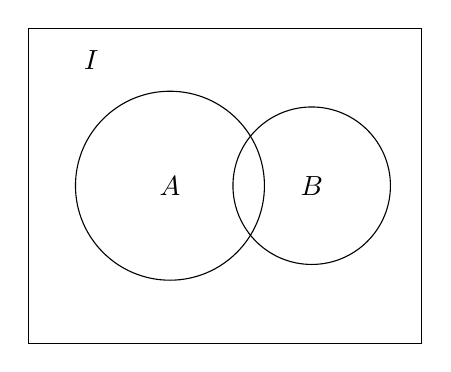
\begin{tikzpicture}
        \draw (0,0) circle (1.2) node{$A$};
        \draw (1.8,0) circle (1.0) node{$B$};
        \draw (-1.8, -2) rectangle (3.2,2);
        \node at (-1,1.6) {$I$};
    \end{tikzpicture}
    \caption*{(1)}
    \end{minipage}
    \qquad
    \begin{minipage}{7cm}
    \centering
    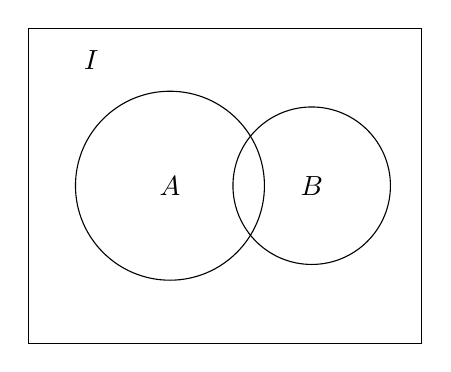
\begin{tikzpicture}
        \draw (0,0) circle (1.2) node{$A$};
        \draw (1.8,0) circle (1.0) node{$B$};
        \draw (-1.8, -2) rectangle (3.2,2);
        \node at (-1,1.6) {$I$};
    \end{tikzpicture}
    \caption*{(2)}
    \end{minipage}
    \caption*{(第11题)}
\end{figure}

\xiaoti{设 $A = \{x \mid x=2k,\ k \in Z\}$,$B = \{x \mid x=2k+1,\ k \in Z\}$,$I=Z$,求$\buji{A}$,$\buji{B}$。}

\end{xiaotis}
